% !TEX program = XeLaTeX
% !TEX encoding = UTF-8
\documentclass[UTF8,nofonts]{article}
%{ctexart}


%\setCJKmainfont[BoldFont=FandolSong-Bold.otf,ItalicFont=FandolKai-Regular.otf]{FandolSong-Regular.otf}
%\setCJKsansfont[BoldFont=FandolHei-Bold.otf]{FandolHei-Regular.otf}
%\setCJKmonofont{FandolFang-Regular.otf}



\usepackage[T1]{fontenc} % recommended for languages with accents
\renewcommand{\refname}{Referencias}




\usepackage{url}
\usepackage{cancel}
\usepackage{xspace}
\usepackage{graphicx}
\usepackage{multicol}
\usepackage{multirow}
\usepackage{subfig}
\usepackage{amsmath}
\usepackage{amssymb}
\usepackage[a4paper, width=186mm, top=18mm, bottom=18mm, includeheadfoot]{geometry}
%\usepackage[a4paper, width=140mm, top=18mm, bottom=22mm, includeheadfoot]{geometry}
\usepackage{booktabs}
\usepackage{array}
\usepackage{verbatim}
\usepackage{caption}
\usepackage{natbib}
\usepackage{booktabs}
\usepackage{float}
\usepackage{pdflscape}
\usepackage{mathtools}
\usepackage[usenames, dvipsnames]{xcolor}
\usepackage{afterpage}
\usepackage{pgf}
\usepackage{tikz}
\usepackage{dirtree}
\usepackage[style=american]{csquotes}
\usepackage{amsfonts}
\usepackage{tikz}
\usepackage{tkz-graph}
\usetikzlibrary{arrows,decorations.pathmorphing,automata,positioning,backgrounds,fit,shapes.symbols,chains,intersections}

\newtheorem{definition}{Definition}[section]
\newtheorem{theorem}{Theorem}[section]
\newtheorem{lemma}{Lemma}
\newtheorem{proof}{Proof} [section]



\usepackage[toc, page, title, titletoc, header]{appendix}
\usepackage{marginnote}
\usepackage{tablefootnote}

%\renewcommand\appendixname{附\ 录}
%\renewcommand\appendixpagename{附\ 录}
%\renewcommand\appendixtocname{附\ 录}
\renewcommand\abstractname{Abstracto}


\usepackage{perpage} %the perpage package
\MakePerPage{footnote} %the perpage package command

\usetikzlibrary{shapes.geometric}%
\usepackage{color}
%\usepackage[pages=some, placement=top]{background}
\usepackage{eso-pic}
\usepackage[final]{pdfpages}

%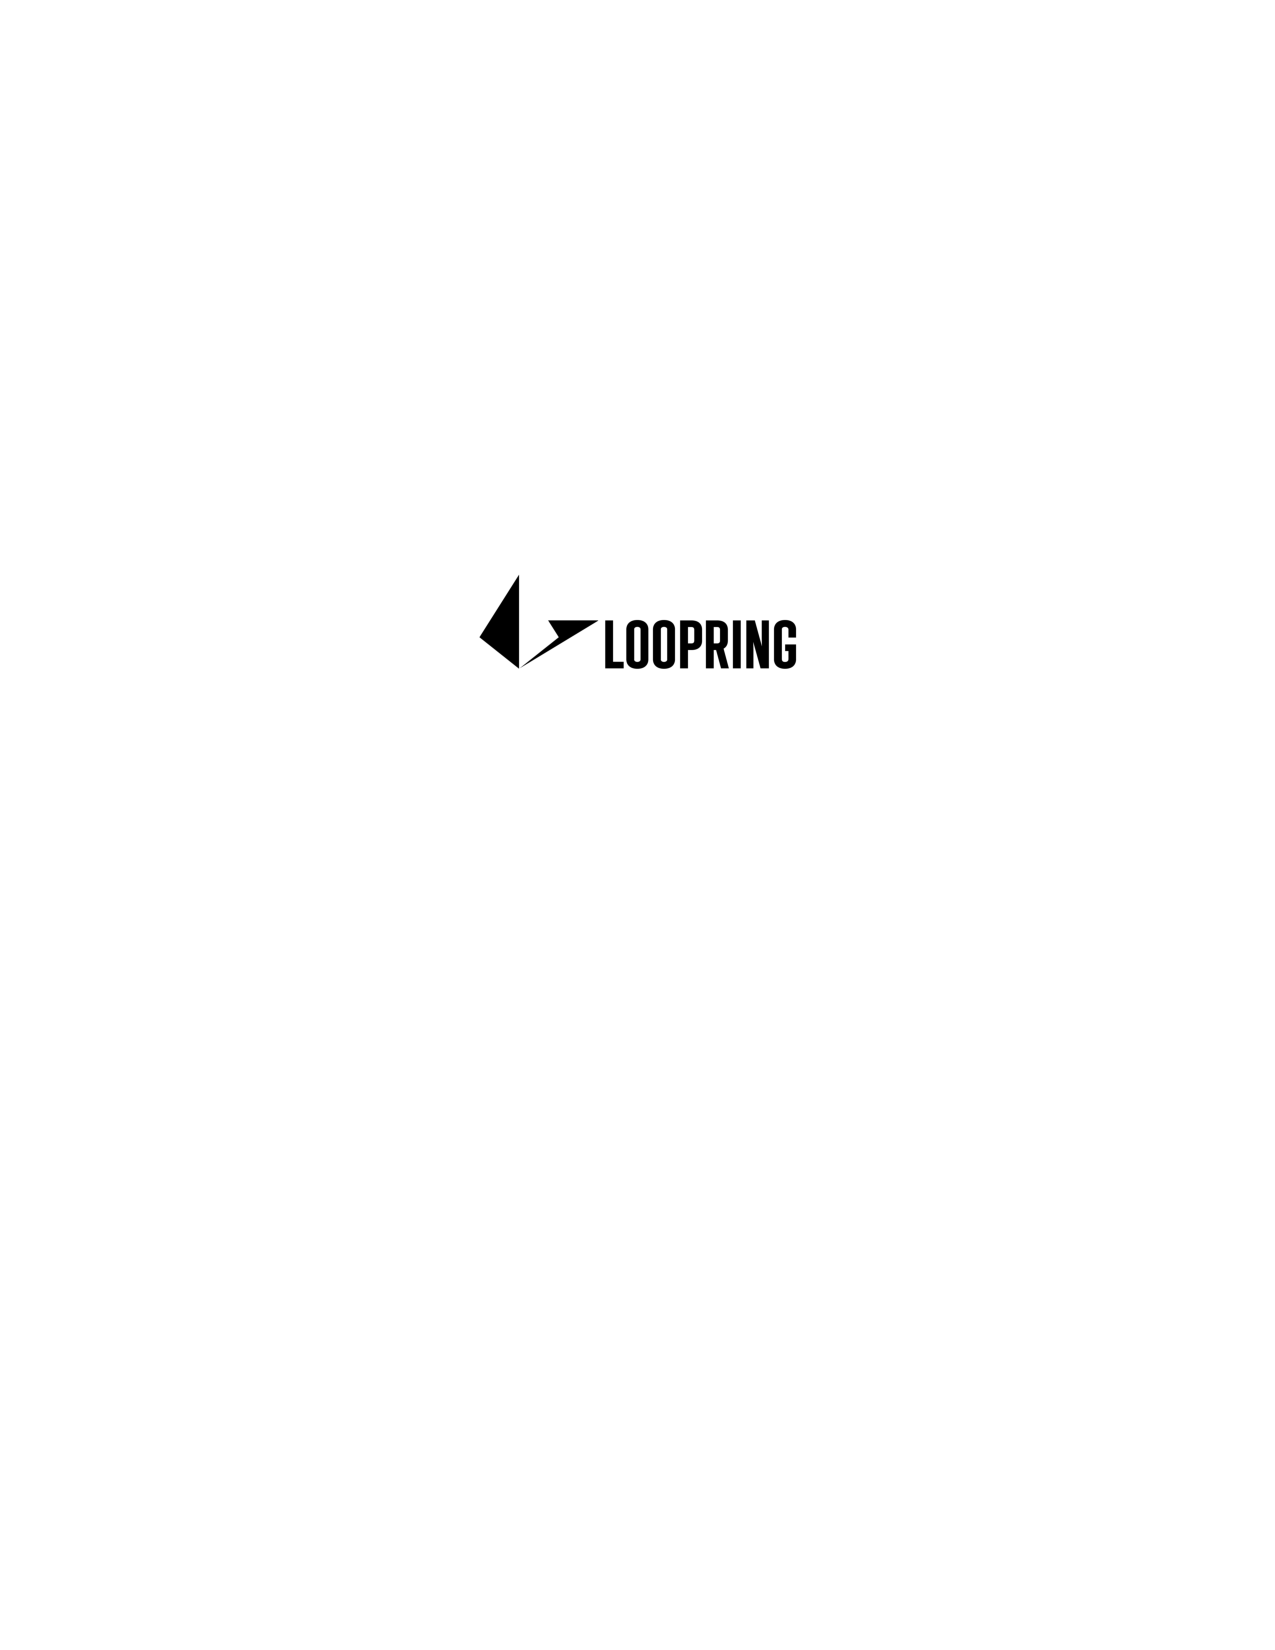
\includepdf[pages=1]{cover}
\hyphenpenalty=750

\title{\textbf{Loopring:}\\\textbf{Un Protocolo de Intercambio de Tokens Decentralizado}}
\author{
  Daniel Wang\\
  \texttt{daniel@loopring.org}\\
  \and
  	Jay Zhou\\
  	\texttt{jay@loopring.org}\\
  	\and
  	Alex Wang\\
  	\texttt{alex@loopring.org}\\
  	\and
  	Matthew Finestone\\
  	\texttt{matt.finestone@gmail.com}\\ 
  \\
  \texttt{https://loopring.org}
 }

\makeatletter
\def\CTEX@section@format{\Large\bfseries}
\makeatother

\makeatletter
\newenvironment{tablehere}
 {\def\@captype{table}}
 {}

\newenvironment{figurehere}
 {\def\@captype{figure}}
 {}
\makeatother
%
%\newcommand\BackgroundPic{%
%\put(0, 0){%
%\parbox[b][\paperheight]{\paperwidth}{%
%\vfill
%\centering
%\includegraphics[width=\paperwidth, height=\paperheight, %
%%keepaspectratio]{images/background.jpg}%
%]{images/background.jpg}%
%\vfill
%}}}


\begin{document}
%\AddToShipoutPicture{\BackgroundPic}
\maketitle


\begin{abstract}
Loopring es un protocolo abierto que construye intercambios descentralizados. Loopring opera como un conjunto p\'ublico de contratos inteligentes (smart contracts) responsables del comercio y la liquidaci\'on, con un grupo de agentes fuera-de-cadena (off-chain) que agregan y comunican \'ordenes. El protocolo es gratuito, extensible, y sirve como un elemento de soporte estandarizado para la construcci\'on de aplicaciones descentralizadas (dApps) que incorporan la funcionalidad de intercambios. Sus est\'andares interoperables facilitan un comercio an\'onimo sin-confianza (trustless). Una mejora importante con respecto a los protocolos de intercambios descentralizados actuales es la habilidad para hacer que las \'ordenes sean mezcladas y combinadas con otras \'ordenes diferentes, obviando las restricciones de formar pares de intercambio entre dos-tokens y mejorando dr\'asticamente la liquidez. Adem\'as, Loopring emplea una soluci\'on \'unica y robusta para la prevenci\'on del front-running: el intento injusto de enviar transacciones a un bloque m\'as r\'apido que el proveedor de la soluci\'on original. Loopring es agn\'ostica en relaci\'on con las cadenas de bloques (blockchains), y puede implantarse en cualquier blockchain con funcionalidad de contrato inteligente. Hasta este momento de escribir este documento, Loopring es operable en Ethereum  \cite{buterin2017ethereum} \cite{wood2014ethereum} y Qtum \cite{dai2017smart} con NEO \cite{atterlonn2018distributed} siendo construida.
\end{abstract}

\begin{multicols}{2}
\section{Introducci\'on\label{sec:introduction}}
Con la proliferaci\'on de activos basados en la blockchain, la necesidad de intercambiar estos activos entre las partes interesadas ha crecido considerablemente.  A medida que miles de nuevos tokens son introducidas - incluyendo los activos tradicionales de tokenizaci\'on -esta necesidad se magnifica. Ya sea intercambiando tokens por motivaciones comerciales especulativas, o convirti\'endose en sus tokens de utilidad nativos para acceder a la red espec\'ifica, la habilidad de intercambiar una cripto a un activo por otro es fundamental para un ecosistema mayor. De hecho, hay una energ\'ia potencial en los activos \cite{desotocapital}, y liberando esta energ\'ia - para desbloquear el capital – no solo requiere determinar la propiedad, que las blockchains han permitido inmutablemente, sino que tambi\'en la habilidad de transferir y transformar libremente estos activos.

Como tal, el intercambiode tokens (valor) que no requieren una relaci\'on de confianza es un caso de uso convincente para la tecnolog\'ia blockchain. Sin embargo, hasta ahora, los entusiastas de la criptograf\'ia se han conformado en gran medida por comerciar tokens en los lugares de intercambio (exchanges, en ingl\'es) centralizados tradicionales.  El protocolo Loopring es necesario porque, al igual que Bitcoin \cite{nakamoto2008bitcoin}, este enfatiza diligentemente que, con respecto al dinero electr\'onico entre-pares (peer-to-peer), \enquote{los mayores beneficios se pierden si un tercero confiable todav\'ia requiere de doble gasto)}, de la misma manera, los principales beneficios de los recursos descentralizados se pierden si tienen que pasar por intercambios de confianza, cerrados y centralizados.

El comercio de tokens descentralizados en los lugares de intercambio o Exchange centralizados no tiene sentido desde el punto de vista filos\'ofico, porque es imposible mantener los valores propugnados por estos proyectos descentralizados. Tambi\'en existen numerosos riesgos pr\'acticos y limitaciones en el uso de exchanges centralizados, que se describir\'an m\'as adelante. Los Exchanges Descentralizados (DEX) \cite{schuh2015bitshares} \cite{bancor} \cite{kyber} han tratado de abordar estos problemas y, en muchos casos, han logrado mitigar los riesgos de seguridad mediante el uso de las blockchains para negociaciones directas. Sin embargo, dado que la capacidad de DEX se convierte en una infraestructura crucial para la nueva econom\'ia, existe un margen considerable para la mejora del rendimiento. Loopring tiene como objetivo proporcionar herramientas modulares para dicha infraestructura con su protocolo abierto de Aplicaciones Decentralizadas (dApp) agn\'osticas.


\section{El panorama actual de las Exchanges\label{sec:current_exchange_landscape}}

\subsection{Insuficiencias de los Exchanges Centralizados}
Los tres principales riesgos asociados con los exchanges centralizados son; 1) falta de seguridad, 2) falta de transparencia, y 3) Falta de liquidez.

\textbf{La falta de seguridad} generalmente surge del hecho de que los usuarios suelen ceder sus llaves privadas (es decir, fondos) a una entidad centralizada. Esto expone a los usuarios a la posibilidad de que los exchanges centralizados sean presa de hackers maliciosos. Los riesgos de seguridad y los ciberataques sufridos por los exchanges son bien conocidos \cite{coincheckhack}  \cite{mcmillan2014inside}, aunque a menudo se aceptan como \enquote{table stakes”} o \enquote{mesa de riesgos}, en el comercio del intercambio de tokens.
    Al tener bajo su custodia a m\'as de millones de d\'olares en fondos de los usuarios, en sus servidores, los exchanges centralizados contin\'uan siendo atractivos para el ataque de los hackers. Adem\'as, los desarrolladores de exchanges pueden cometer errores accidentales, honestos, con los fondos de los usuarios. Simplemente, los usuarios no tienen el control de sus tokens cuando los depositan en un exchange centralizado.

\textbf{La falta de transparencia} expone a los usuarios al riesgo de que los exchanges deshonestos act\'uen injustamente o incorrectamente. La distinci\'on aqu\'i se basa en las intenciones maliciosas de los operadores de los exchanges, ya que los usuarios no est\'an realmente comerciando sus propios activos en estos exchanges centralizados, sino m\'as bien, hacen un \enquote{reconocimiento de la deuda} (IOU). Cuando los tokens son enviados a la billetera del exchange, el exchange los pone bajo su custodia y ofrece un reconocimiento de la deuda (IOU) en su lugar. Es as\'i como, todos los intercambios de comercio se realizan entre los pagar\'es-IOU de los usuarios. Para retirar, los usuarios canjean sus pagar\'es-IOU con el exchange, y reciben sus tokens en la direcci\'on de su billetera externa. En este proceso hay una falta de transparencia, y el exchange puede cerrar, congelar su cuenta, declararse en quiebra, etc. Tambi\'en existe la posibilidad de que utilicen los activos de los usuarios para otros fines mientras los mantienen bajo su custodia, como prestarlos a terceros. La falta de transparencia puede tener un costo para los usuarios, aun as\'i, sin perder el total de fondos, por ejemplo, puede generar tasas de cambio m\'as altas, retrasos en los momentos de mayor demanda, riesgos regulatorios y \'ordenes siendo “front-ran” (transacciones enviadas a un bloque m\'as r\'apido que el proveedor de la soluci\'on original)

\textbf{Falta de liquidez.} Desde el punto de vista de los operadores del exchange, la liquidez fragmentada impide la entrada de nuevos exchanges debido a la presencia de dos escenarios del \enquote{el-ganador-se-lleva-todo”}. En el primero, el exchange con el mayor n\'umero de pares de divisas gana, porque a los usuarios les resulta m\'as ventajoso realizar todos sus intercambios comerciales en un solo exchange. En el segundo, el exchange con el mayor registro de \'ordenes gana, debido al diferencial favorable del bid-ask (oferta-demanda) para cada uno de los pares de intercambio. Esto desalienta la competencia de las personas nuevas en el mercado de intercambios porque les resulta dif\'icil acumular la liquidez inicial necesaria. Como resultado, es que muchos exchanges controlan una gran parte del mercado a pesar de las quejas de los usuarios y los incidentes sustanciales de ciberataques por hackers inform\'aticos. Es importante subrayar que cuanto los exchanges centralizados m\'as compren y ganen las cuotas del mercado, m\'as expuestos est\'an a los ataques de hackers.

Desde el punto de vista de los usuarios, la fragmentaci\'on de la liquidez reduce considerablemente la experiencia del usuario en su facilidad de uso. En un exchange centralizado, los usuarios solo pueden comerciar dentro de los grupos de liquidez de los exchanges, contra sus propios libros mayores y entre los pares de tokens que soporta. Para intercambiar el token \verb|A| por el token \verb|B|, los usuarios deben ir a un exchange que soporte ambos tokens o registrarse en diferentes exchanges, divulgando su informaci\'on personal. Los usuarios a menudo necesitan realizar transacciones preliminares o intermedias, generalmente mediante BTC o ETH, pagando las brechas entre la oferta y la demanda en el proceso. Finalmente, los libros mayores pueden no ser lo suficientemente grandes como para completar la transacci\'on sin una desaceleraci\'on importante. Incluso si el exchange afirma que puede manejar grandes vol\'umenes, no hay garant\'ia de que este volumen y liquidez no sean falsos \cite{fakevolume}.

Los resultados son silos de liquidez desconectados y un ecosistema fragmentado que se asemeja al antiguo sistema financiero, con un volumen significante de transacciones centralizadas en unos pocos exchanges. Las promesas de liquidez global de las blockchains no tienen ning\'un m\'erito o valor dentro de los exchanges centralizados.

\subsection{Insuficiencias de los Exchanges descentralizados}
Los exchanges descentralizados se diferencian de los exchanges centralizados, en parte porque los usuarios mantienen el control de sus llaves-privadas (activos) mediante la ejecuci\'on directa de intercambios en la blockchain subyacente. Aprovechando la \enquote{tecnolog\'ia sin confianza} de las criptomonedas, ellas mismas han mitigado con \'exito muchos de los riesgos en torno a la seguridad antes mencionados. Sin embargo, los problemas persisten en relaci\'on con el rendimiento y las limitaciones estructurales.

La liquidez a menudo sigue siendo un problema, ya que los usuarios deben buscar contrapartes a trav\'es de grupos de liquidez y est\'andares dispares. Los efectos de la liquidez fragmentada est\'an presentes si los DEXs o dApps no utilizan est\'andares consistentes para interoperar, y si las \'ordenes no son compartidas o propagadas dentro de una red amplia. La liquidez del limite de los libros mayores, y, espec\'ificamente, su capacidad de recuperaci\'on, cu\'an r\'apido las \'ordenes de limite ejecutadas son reemplazadas por \'ordenes nuevas -  puede afectar significantemente a las estrategias optimas de intercambio \cite{limitorderliquidity}. La ausencia de estos est\'andares ha resultado no solo en la reducci\'on de la liquidez, sino tambi\'en en la exposici\'on a una variedad de contratos inteligentes patentados potencialmente inseguros.

Adem\'as, dado que los intercambios se realizan en cadena, los DEX heredan las limitaciones de la bloackchain subyacente, nominalmente: escalabilidad, retrasos en la ejecuci\'on (proceso de miner\'ia) y modificaciones costosas en las \'ordenes. Por lo tanto, el registro de \'ordenes de la blockchain no se escala particularmente bien, ya que la ejecuci\'on de c\'odigo en la blockchain genera un costo (gas), lo que hace que las cancelaciones m\'ultiples de \'ordenes sean excesivamente caras.

Finalmente, dado que los registros de las \'ordenes de la blockchain son p\'ublicos, la transacci\'on para hacer una orden es visible para los mineros de criptomedas, mientras se espera que sea extra\'ida en el bloque siguiente y colocada en libro mayor. Este retraso expone a los usuarios al riesgo de una \enquote{ejecuci\'on anticipada} (front-run) y tambi\'en al riesgo de tener el precio o la ejecuci\'on en su contra.

\subsection{Soluciones H\'ibridas}
Por las razones mencionadas anteriormente, los exchanges puramente basados en blockchain tienen limitaciones que los hacen no competitivos con los exchanges centralizados. Existe un balance entre la falta de confianza caracter\'istica de la en-cadena (on-chain, en ingl\'es) y la velocidad y flexibilidad de las \'ordenes de exchanges centralizadas. Protocolos como los de Loopring y 0x  \cite{warren20170x} proponen una soluci\'on de liquidaci\'on de transacciones en-cadena con una gesti\'on de \'ordenes fuera de l\'inea. Estas soluciones giran en torno a los contratos inteligentes abiertos, pero superan las limitaciones de escalabilidad mediante la ejecuci\'on de muchas funciones fuera de la cadena (off-chain, en ingl\'es) y dejando a los nodos flexibilidad para completar diferentes roles cr\'iticos para la red. Sin embargo, las desventajas tambi\'en permanecen para los modelos h\'ibridos  \cite{costofdecent}. El protocolo Loopring propone diferencias significativas, nuestro enfoque para una soluci\'on h\'ibrida se presenta a trav\'es de este art\'iculo.

\section{El protocolo Loopring\label{sec:loopring_protocol}}
Loopring no es un Exchange descentralizado (DEX), sino un protocolo modular para construir DEXs en m\'ultiples blockchains. Hemos desmontado partes de los componentes principales de una exchange tradicional y hemos ofrecido un conjunto de contractos inteligentes p\'ublicos y agentes descentralizados en su lugar. Los roles en la red incluyen billeteras, rel\'es (relays, en ingl\'es), blockchains de consorcio para compartir liquidez, buscadores de registros de \'ordenes, Mineros-de-anillo (Ring-miners, en ingl\'es) y servicios de tokenizaci\'on de activos. Antes de definir cada uno de estos elementos, primero debemos entender cu\'ales son las \'ordenes en Loopring.

\subsection{Anillo de \'Ordenes \label{sec:order_ring}}
Las \'ordenes en Loopring se expresan en lo que llamamos el Modelo de Orden Unidireccional (UDOM)\cite{coinport2014udom}. La UDOM expresa \'ordenes como solicitudes de intercambio de token, \verb|cantidadS|/\verb|cantidadB|, (cantidad para vender / comprar) en lugar de las \'ordenes de oferta y demanda. Dado que cada orden es solo un tipo de cambio entre dos tokens, una caracter\'istica importante del protocolo es la mezcla y coincidencia entre varias \'ordenes en un intercambio circular. Utilizando hasta 16 \'ordenes simult\'aneamente en lugar de un solo par de intercambio, se genera un aumento dr\'astico en la liquidez y un potencial para la mejora del precio.

\begin{center}
\begin{figurehere}
\centering
\tikzstyle{block} = [draw, fill=blue!20, rectangle, 
    minimum height=3em, minimum width=6em]
\tikzstyle{sum} = [draw, fill=blue!20, circle, node distance=1cm]
\tikzstyle{input} = [coordinate]
\tikzstyle{output} = [coordinate]
\tikzstyle{pinstyle} = [pin edge={to-,thin,black}]

\begin{tikzpicture}[
    auto, 
    node distance=2cm,
    >=latex',
    font=\bfseries\footnotesize\sffamily,
    order/.style={
		scale=0.7,
		rectangle,
		rounded corners,
		draw=black, 
		text centered,
%		text width=5cm,
		minimum height=12mm,
		fill=white
	},
	label/.style={
		scale=0.7
	}
  ]
    % We start by placing the blocks

  \node [order] (order2) 
 {%
 \begin{tabular}{l}
  \textbf{ORDEN\#2}\\
  \textbf{propietario: Y}\\
  \textbf{cantidadS: 9B}\\
  \textbf{cantidadB: 12C}
 \end{tabular}
 };
 
  \node [order, below of=order2, xshift=-3.5cm] (order1) 
 {%
 \begin{tabular}{l}
  \textbf{ORDEN\#1}\\
  \textbf{propietario: X}\\
  \textbf{cantidadS: 10000A}\\
  \textbf{cantidadB: 2B}
 \end{tabular}
 };
 
 
  \node [order, below of=order2, xshift=3.5cm] (order3) 
 {%
 \begin{tabular}{l}
  \textbf{ORDEN\#3}\\
  \textbf{propietario: Z}\\
  \textbf{cantidadS: 100C}\\
  \textbf{cantidadB: 160A}
 \end{tabular}
 };
 
 \draw [draw,->] (order1) -- node [label] {\textbf{7898A}} (order3);
 \draw [draw,->] (order2) -| node [label, xshift=-1.8cm] {\textbf{8B}} (order1);
 \draw [draw,->] (order3) |- node [label, xshift=1cm, yshift=0.24cm] {\textbf{98C}} (order2);

\end{tikzpicture}

\caption{Un anillo de orden de 3 \'ordenes}
\label{fig:ring}
\end{figurehere}
\end{center}

La figura de arriba muestra un anillo de \'ordenes de 3 \'ordenes. El token de cada orden para vender (\verb|tokenS|) es el token de otra orden para comprar (\verb|tokenB|). Esto crea un bucle que permite que cada orden intercambie sus tokens deseados sin necesidad de una orden opuesta a su par. Los pares de \'ordenes comerciales tradicionales pueden, por supuesto, seguir ejecut\'andose, en lo que es esencialmente un caso especial de un anillo de \'ordenes.

\begin{definition}[anillo-de-\'ordenes] Deje $C_{0}$, $C_{1}$, $\cdots$, $C_{n-1}$ ser $n$ diferentes tokens, $O_{0\rightarrow 1}$, $\cdots$, $O_{i\rightarrow i\oplus 1}$, $\cdots$, $O_{n-1 \rightarrow 0}$ ser $n$ \'ordenes. Estas \'ordenes pueden formar un anillo-de-\'ordenes para intercambiar:
$$O_{0\rightarrow 1} \rightarrow \cdots \rightarrow O_{i\rightarrow i\oplus 1} \rightarrow \cdots \rightarrow O_{n-1\rightarrow 0} \text{, }$$
donde $n$ es la longitud de la orden-anillo, y $i\oplus 1 \equiv i+1 \mod n$.
\end{definition}

Un anillo de \'ordenes es v\'alido cuando todas las transacciones que lo componen se pueden realizar a un tipo de cambio igual o superior a la tasa original especificada por el usuario. Para verificar la validez del anillo de \'ordenes, los contratos inteligentes del protocolo Loopring deben recibir los anillos de \'ordenes de los mineros y verificar que el producto de las tasas de cambio originales de todas las \'ordenes sea mayor o igual a 1.

Supongamos que Alice y Bob quieren intercambiar sus token \verb|A| y \verb|B|. Alice tiene 15 token \verb|A| y quiere 4 token \verb|B|; Bob tiene 10 token \verb|B| y quiere 30 token \verb|A| a cambio de sus tokens.


?`Qui\'en est\'a comprando y qui\'en est\'a vendiendo? Esto depende solo en los activos que necesitamos fijar para dar las cotizaciones de precios. Si token \verb|A| es la referencia, entonces Alice est\'a comprando token \verb|B| por el precio de ${15 \over 4} = 3.75$\verb|A|, mientras que Bob vende 10 token \verb|B| por el precio de ${30 \over 10} = 3.00$\verb|A|. En el caso de la fijaci\'on de token \verb|B| como referencia, decimos que Alice est\'a vendiendo 15 token \verb|A| por el precio de ${4 \over 15} = 0.26666667$\verb|B| y Bob est\'a comprando 10 token \verb|A| por el precio de ${10 \over 30} = 0.33333334 $\verb|B|. Por lo tanto, qui\'en es el comprador o el vendedor es arbitrario.

En la primera situaci\'on, Alice est\'a dispuesta a pagar un precio m\'as alto ($3.75$\verb|A|) que el precio por el que Bob est\'a vendiendo sus token ($3.00$\verb|A|), mientras que en la segunda situaci\'on Bob est\'a dispuesto a pagar un precio m\'as alto ($ 0.33333334 $\verb|B|) que el precio por el que Alice est\'a vendiendo sus tokens ($ 0.26666667 $\verb|B|). Est\'a claro que un intercambio es posible siempre que el comprador est\'e dispuesto a pagar un precio igual o superior al precio del vendedor.

\begin{equation}
{{15\over 4} \over {30\over 10}} = {{10\over 30} \over {4\over 15}}={15 \over 4} \cdot {10 \over 30} = 1.25 > 1
\end{equation}

Por lo tanto, para que un conjunto de $n$ \'ordenes puedan ser llenadas y ejecutadas, total o parcialmente, necesitamos saber si el producto de cada una de las tasas de cambio como \'ordenes de compra resulta en un n\'umero mayor o igual a 1. Si es as\'i, todas las \'ordenes $n$ pueden estar parcialmente, o totalmente ejecutadas \cite {supersymmetry}.

Si presentamos a un tercer participante, Charlie, as\'i que si Alice quiere dar $x_1$ token \verb|A| y recibe $y_1$ token \verb|B|, Bob quiere dar $x_2$ token \verb|B| y recibe $y_2$ token \verb|C|, y Charlie quiere dar $x_3$ token \verb|C| y recibir $y_3$ token \verb|A|. Los tokens necesarios est\'an presentes, y el intercambio es posible si:

\begin{equation}
{{x_1 \cdot x_2 \cdot x_3 \over y_1 \cdot y_2 \cdot y_3} \geq 1}
\end{equation}



Ver la secci\'on \ref{anatomy} para m\'as detalles referentes a las \'ordenes de Loopring.

\section{Participantes del Ecosistema\label{sec:ecosystem}}
Los siguientes participantes del ecosistema proporcionan conjuntamente todas las funcionalidades que un exchange centralizado ofrece.
\begin{itemize}


\item \textbf{Billeteras}: Un servicio o interfaz de la billetera que permite a los usuarios acceder a sus tokens y a enviar \'ordenes a la red de Loopring. Las billeteras ser\'an incentivadas a producir \'ordenes al compartir pagos dentro del anillo de \'ordenes (ver secci\'on \ref{sec:token}). Con la creencia de que el futuro de la negociaci\'on tendr\'a lugar dentro de la seguridad de las billeteras de los usuarios individuales, la conexi\'on de estos fondos de liquidez a trav\'es de nuestro protocolo es primordial.

\item \textbf {Blockchain de consorcio para  intercambio de liquidez /Malla-Rel\'e}: una red de malla de rel\'e (relay mesh network, en ingl\'es) para el intercambio de \'ordenes \& liquidez. Cuando los nodos ejecutan el software de rel\'e de Loopring, ellos pueden unirse a una red existente y compartir liquidez con otros rel\'es a trav\'es de una blockchain de consorcio. La blockchain de consorcio que estamos construyendo como primera implementaci\'on tiene un tiempo casi real de intercambio de \'ordenes (bloques de 1-2 segundos), y reduce el historial antiguo para permitir a los nuevos nodos una descarga m\'as r\'apida. Notablemente, los rel\'es no necesitan unirse a este consorcio; pueden actuar solos y no compartir liquidez con otros, o pueden comenzar y administrar su propia red de intercambios de liquidez.

\item \textbf{Rel\'es / Mineros-de-anillos}: Los rel\'es son nodos que reciben \'ordenes de las billeteras o de la malla de rel\'es, mantienen un registro p\'ublico de \'ordenes y uno de comercio, y opcionalmente emiten \'ordenes a otros rel\'es (a trav\'es de cualquier medio de fuera-de-cadena arbitraria) y/o nodos de malla de retransmisi\'on. La miner\'ia de anillo es una caracter\'istica -- no un requisito -- de los rel\'es. Es computacionalmente intensa y se realiza completamente fuera-de-cadena (off-chain). Llamamos a los rel\'es con la funci\'on activada de miner\'ia de anillo \enquote{Ring-Miners}, que producen anillos de \'ordenes al unir \'ordenes dispares. Los rel\'es son libres de (1) c\'omo elegir comunicarse entre ellos, (2) c\'omo construir sus libros mayores, y (3) c\'omo extraer anillos de \'ordenes (algoritmos de miner\'a).

\item \textbf{Contratos inteligentes del protocolo Loopring (LPSC)}: Un conjunto de contratos inteligentes p\'ublicos y gratuitos que verifican los anillos de \'ordenes recibidos de los mineros de anillo (ring-miners), transfieren los tokens en nombre de los usuarios de manera segura, incentivan las operaciones de las billeteras y de los mineros con comisiones, y crean eventos. Los rel\'es (relays) /navegadores de \'ordenes escuchan estos eventos para mantener sus libros mayores y su historial comercial actualizados. Ver ap\'endice \ref{app:protocol_ethereum} para m\'as detalles.

\item \textbf{Servicios de tokenizaci\'on de activos (ATS)}: un puente entre activos que no pueden intercambiarse directamente en Loopring. Estos servicios son administrados centralmente por empresas y organizaciones acreditadas. Los usuarios depositan activos (activos reales, fiat o token de otras blockchains) y obtienen tokens que pueden ser redimidos para sus dep\'ositos en el futuro. Looping no es un protocolo de intercambio de cadena-cruzada/cross-chain (hasta que se encuentre una soluci\'on adecuada), pero los servicios de tokenizaci\'on de activos (ATS) permiten el intercambio entre tokens ERC20 \cite{ERC20} y recursos f\'isicos, as\'i como con los recursos presentes en otras blockchains.

\end{itemize}



\section{Proceso de Exchange/Intercambio\label{sec:process}}
\begin{enumerate} 

\item \textbf{Autorizaci\'on del protocolo}: En la figura \ref{fig:process}, el usuario \verb|Y|, quien quiere intercambiar tokens, autoriza a los LPSC a administrar una \verb|cantidadS| del token \verb|B| que el usuario quiere vender. Esta operaci\'on no bloquea los tokens del usuario, quien puede transferirlos libremente mientras se procesa la orden.

\item \textbf{Creaci\'on de la orden}: El tipo de cambio actual y el registro de \'ordenes del token \verb|B| vs token \verb|C|, son proporcionados por rel\'es o por otros agentes conectados a la red, como los buscadores de \'ordenes. El usuario \verb|Y| hace una orden (orden con l\'imite de precio) especificando  \verb|cantidadS| y \verb|cantidadB| y otros par\'ametros a trav\'es de cualquier interface de billetera integrada. Cierta cantidad de LRx se puede agregar a la orden como una comisi\'on para los mineros de anillo (ring-miners); cu\'an mayor sea la comisi\'on de LRx, mayor ser\'a la probabilidad de que un minero procese r\'apidamente la orden. El hash de la orden se firma con la clave privada del usuario \verb|Y|.

\item \textbf{Transmisi\'on de \'ordenes}: la billetera env\'ia la orden y su firma a uno o m\'as rel\'es (relays, en ingl\'es). Luego los rel\'es actualizan su libro mayor p\'ublico. El protocolo no requiere que los libros mayores sean construidos de una manera espec\'ifica, como por ejemplo con la regla de  \textit{por orden de llegada}, el primero en llegar es el primero en ser atendido. En cambio, los rel\'es tienen el poder de tomar sus propias decisiones de dise\~no mediante la construcci\'on de sus libros mayores.

\item \textbf{Distribuci\'on de liquidez}: los rel\'es transmiten una orden a los otros rel\'es a trav\'es del m\'etodo que consideren m\'as adecuado. De nuevo, hay flexibilidad sobre c\'omo interact\'uan los nodos. Para facilitar el logro de un cierto nivel de conectividad, se ha implementado un mecanismo incorporado para compartir la liquidez entre las mallas de rel\'es (relay-mesh) utilizando un consorcio de blockchains. Como se mencion\'o en la secci\'on anterior, esta malla de rel\'e est\'a optimizada para la velocidad y la inclusi\'on.

\begin{center}
\begin{figurehere}
\centering
\tikzstyle{block} = [draw, fill=blue!20, rectangle, 
    minimum height=3em, minimum width=6em]
\tikzstyle{sum} = [draw, fill=blue!20, circle, node distance=1cm]
\tikzstyle{input} = [coordinate]
\tikzstyle{output} = [coordinate]
\tikzstyle{pinstyle} = [pin edge={to-,thin,black}]

\begin{tikzpicture}[
    auto, 
    scale=0.7,
    node distance=2.2cm, %CHANGED ring-mining Order1 height%
    >=latex',
    font=\bfseries\footnotesize\sffamily,
    order/.style={
		rectangle,
		scale=0.7,
		rounded corners,
		draw=black, 
		text centered,
%		text width=5cm,
		minimum height=12mm,
		minimum width=30mm,
		fill=white
	},
	role/.style={
		circle,
		scale=0.7,
		draw=black, 
		text centered,
%		text width=5cm,
		minimum height=12mm,
		minimum width=12mm,
		fill=white
	},
	steps/.style={
		circle,
		scale=0.7,
		draw=black, 
		text centered,
%		text width=5cm,
%		minimum height=12mm,
%		minimum width=12mm,
		fill=black,
		text=white
	},
	account/.style={
		circle,
		scale=0.7,
		draw=black, 
		text centered,
%		text width=5cm,
		minimum height=16mm,
		minimum width=16mm,
		fill=white
	},
	label/.style={
	  scale=0.7
    }
  ]

 
 \node [role] (user1)  {usuario X};
 \node [role, below of=user1] (user2)  {usuario Y};
 \node [role, below of=user2] (user3)  {usuario Z};
 \node [role, below of=user3, fill=gray!20] (relay1)  {rel\'e M};
 \node [role, below of=relay1, fill=gray!20] (relay2)  {rel\'e N};

 
 \node [order, left of=user1, xshift=-1cm] (order1) 
 {%
 \begin{tabular}{l}
  \textbf{ORDEN 1}\\
  \textbf{propietario: X}\\
  \textbf{cantidadS: 10000 A}\\
  \textbf{cantidadB: 2 B}
 \end{tabular}
 };
 
 \draw [draw, ->]  (user1) -- (order1) [label]{};
 \draw [bend right,->] (order1) to node [auto, scale=0.7] {} (relay1);
 \draw [bend right,->] (order1) to node [auto, scale=0.7] {} (relay2);
% \draw [draw, ->]  (order1) |- (relay1) [label]{};
% \draw [draw, ->]  (order1) |- (relay2) [label]{};
 
 \node [order,left of=user2, xshift=-1.5cm] (order2) 
 {%
 \begin{tabular}{l}
  \textbf{ORDEN 2}\\
  \textbf{propietario: Y}\\
  \textbf{cantidadS: 9  B}\\
  \textbf{cantidadB: 12 C}
 \end{tabular}
 };
 \draw [draw, ->]  (user2) -- (order2) [label]{};
 \draw [bend right,->] (order2) to node [auto, scale=0.7] {} (relay1);
 \draw [bend right,->] (order2) to node [auto, scale=0.7] {} (relay2);
% \draw [draw, ->]  (order2) |- (relay1) [label]{};
% \draw [draw, ->]  (order2) |- (relay2) [label]{};
% 
\node [order, left of=user3, xshift=-2cm] (order3) 
 {%
 \begin{tabular}{l}
  \textbf{ORDEN 3}\\
  \textbf{propietario: Z}\\
  \textbf{cantidadS: 100 C}\\
  \textbf{cantidadB: 160 A}
 \end{tabular}
 };
 \draw [draw, ->]  (user3) -- (order3) [label]{};
 \draw [bend right,->] (order3) to node [auto, scale=0.7] {} (relay1);
 \draw [bend right,->] (order3) to node [auto, scale=0.7] {} (relay2);
% \draw [draw, ->]  (order3) |- (relay1) [label]{};
% \draw [draw, ->]  (order3) |- (relay2) [label]{};
 
% // The Ring
\node [order, 
yshift=-1.5cm,
xshift=-2.75cm,
below of=relay2,
fill=gray!10,
minimum width=4.2cm,
minimum height=5.4cm] (ring) {}; %changed size%


\node [order, dashed, below of=relay2,yshift=-0.2cm,xshift=-2.5cm] (order11) 
 {%
 \begin{tabular}{l}
  \textbf{ORDEN 1}\\
  \textbf{propietario: X}\\
  \textbf{cantidadS: 10000 A}\\
  \textbf{cantidadB: 2 B}
 \end{tabular}
 };
 \node [order, dashed,below of=order11,xshift=-0.25cm,yshift=0.7cm] (order21) 
 {%
 \begin{tabular}{l}
  \textbf{ORDEN 2}\\
  \textbf{propietario: Y}\\
  \textbf{cantidadS: 9  B}\\
  \textbf{cantidadB: 12 C}
 \end{tabular}
 };
\node [order, dashed,below of=order21,xshift=-0.25cm,yshift=0.7cm] (order31) 
 {%
 \begin{tabular}{l}
  \textbf{ORDEN 3}\\
  \textbf{propietario: Z}\\
  \textbf{cantidadS: 100 C}\\
  \textbf{cantidadB: 160 A}
 \end{tabular}
 };
 
 % // The blockchain
\node [
rectangle,
fill=gray!20, 
right of=user1,
yshift=-4.5cm,
xshift=0.1cm,
scale=0.7,
minimum width=3.2cm,
minimum height=15.6cm] (blockchain) {\parbox[b][15cm]{1.3cm}{blockchain}};
% blockchain accounts
  \node [account, right of=user1, xshift=1cm] (account1)  {cuentaX};
  \node [account, right of=user2, xshift=1cm] (account2)  {cuentaY};
  \node [account, right of=user3, xshift=1cm] (account3)  {cuentaZ};
  \node [account, right of=relay1, xshift=1cm] (account4)  {cuentaM};
  \node [account, right of=relay2, xshift=1cm] (account5)  {cuentaN};
  \node [account, double, below of=account5, yshift=-1.5cm] (psc)  {LPSC};
  
 \draw [draw, ->]  (user1) -- (account1) [label]{};
 \draw [draw, ->]  (user2) -- (account2) [label]{};
 \draw [draw, ->]  (user3) -- (account3) [label]{};
% \draw [draw, ->]  (relay1) -- (account4) [label]{};
% \draw [draw, ->]  (relay2) -- (account5) [label]{};
 \draw [draw, double, thick]  (relay1) to node [auto, scale=0.7] {compartir liquidez}  (relay2) [label]{};
% \draw [draw, ->]  (relay1) -- (ring) [label]{};
 \draw [draw, ->]  (relay2) to node [auto, scale=0.7, xshift=-2.3cm, yshift=0.3cm] {miner\'ia de anillo}  (ring) [label]{};
 \draw [draw, ->]  (ring) to node [auto, scale=0.7] {enviarAnillo} (psc) [label]{};
 
 \draw [bend left,->] (account1) to node [auto, scale=0.7] {\textbf{7898 A}} (account3);
 \draw [bend left,->] (account2) to node [auto, scale=0.7] {\textbf{8 B}} (account1);
 \draw [bend left,->] (account3) to node [auto, scale=0.7] {\textbf{98 C}} (account2);
 
 \draw [bend left,->, dashed] (account1) to node [auto, scale=0.7] {} (account5);
 \draw [bend left,->, dashed] (account2) to node [auto, scale=0.7] {} (account5);
 \draw [bend left,->, dashed] (account3) to node [auto, scale=0.7, xshift=.5cm] {\textbf{comisi\'on}} (account5);
  
  
% \draw [draw,->] (order1) -- node [label] {\textbf{7898 A}} (order3);
% \draw [draw,->] (order2) -| node [label, xshift=-1.8cm] {\textbf{8 B}} (order1);
% \draw [draw,->] (order3) |- node [label, xshift=1cm, yshift=0.24cm] {\textbf{98 C}} (order2);

\node [steps, right of=user2, xshift=-0.6cm] () {1};
\node [steps, left of=user2, xshift=0.8cm] () {2};
\node [steps, left of=relay2, xshift=0.3cm, yshift=1cm] () {3};
\node [steps, left of=relay1, xshift=3.3cm, yshift=-1.6cm] () {4};
\node [steps, below of=relay2, xshift=-0.2cm, yshift=0.4cm] () {5};
\node [steps, right of=account3, xshift=-0.6cm] (step5) {6};

 \draw [bend right, ->]  (psc) to node [auto, scale=0.7, xshift=0.5cm] {liquidaci\'on} (step5) [label]{};
 
\end{tikzpicture}

\caption{Proceso de Intercambio de Loopring}
\label{fig:process}
\end{figurehere}
\end{center}

\item \textbf{Miner\'ia de anillo (emparejando \'ordenes)}:  los mineros de anillo intentan ejecutar la orden total o parcialmente a un tipo de tasa de intercambio o mejor, emparej\'andolo con otras \'ordenes m\'ultiples. La miner\'ia de anillo es la raz\'on principal por la cual el protocolo puede proporcionar alta liquidez sobre cualquier otro par. Si la velocidad a la que se ejecuta la orden es mejor que la especificada por el usuario \verb|Y|, el margen se comparte entre todas las \'ordenes que forman el anillo. Como recompensa, el minero puede elegir entre reclamar una parte del margen (Divisi\'on de margen, y devolver a los usuarios el LRx), o simplemente quedarse con la comisi\'on en LRx.


\item \textbf{Verificaci\'on \& transacci\'on}: Los LPSC reciben el anillo de \'ordenes. Se necesitan varios controles para verificar los datos proporcionados por el minero de anillo y para determinar si el ciclo de \'ordenes puede completarse completamente o parcialmente (dependiendo en la tasa de ejecuci\'on de las \'ordenes en el anillo y los tokens en las billeteras de los usuarios). Si todos los controles son exitosos, el contrato autom\'aticamente transfiere los tokens a los usuarios y paga a los mineros de anillo y a las billeteras al mismo tiempo. Si los LPSC detectan la falta de fondos necesarios para el intercambio en la billetera del usuario \verb|Y|, la orden ser\'a reducida: una orden de escala reducida volver\'a autom\'aticamente a su tama\~no original si se deposita una cantidad suficiente de fondos a la direcci\'on del usuario, a diferencia de una cancelaci\'on, que es una operaci\'on manual en un solo sentido que no se puede cancelar.


\end{enumerate}





%
%\end{multicols}
%
%\begin{center}
%\begin{figurehere}
%\includegraphics[height=8cm]{images/en_protocol.png}
%\caption{Loopring Trading Process}
%\label{fig: Loopringrotocol}
%\end{figurehere}
%\end{center}
%
%\begin{multicols}{2}


\section{Flexibilidad operacional\label{sec:business_model}}
Es importante tener en cuenta que los est\'andares abiertos de Loopring permiten a los participantes operar con gran flexibilidad. Los participantes son libres de implementar nuevos modelos de negocio y generar valor para los usuarios, ganando comisiones en LRx en vol\'umenes de negociaci\'on u otras m\'etricas definidas en el proceso (si as\'i lo deciden). El ecosistema es modular y est\'a dise\~nado para fomentar la participaci\'on de una multitud de aplicaciones.

\subsection{Registro de \'ordenes \label{sec:order_book}}
Los rel\'es pueden dise\~nar sus libros mayores en cualquier n\'umero de maneras para mostrar y hacer coincidir las \'ordenes de los usuarios. Una primera implementaci\'on de nuestro libro mayor sigue un modelo de venta-libre (Over The Counter - OTC, en ingl\'es), donde las \'ordenes limitas se basan solo en el precio. El momento en el que se generaron las \'ordenes, en otras palabras, no tiene un impacto en la formaci\'on del libro mayor. Sin embargo, un rel\'e es libre de dise\~nar su propio libro mayor en la manera que se pueda imitar y competir con el funcionamiento t\'ipico de los exchanges centralizados, donde las \'ordenes se clasifican por precio, mientras tambi\'en se respeta el momento de creaci\'on de la orden. Si un rel\'e est\'a m\'as inclinado a ofrecer este tipo de libro mayor, ellos pueden apropiarse/ integrarse con una billetera, y hacer que las \'ordenes desde esa billetera se env\'ien \'unicamente a un solo rel\'e, que luego podr\'a ordenarlos en base al tiempo. Cualquier tipo de configuraci\'on es posible. 
Mientras que otros protocolos DEX a veces requieren de Rel\'es para tener recursos - saldos de tokens iniciales para colocar \enquote{\'ordenes tomadoras} (taker orders, en ingl\'es) - Los rel\'es de Looping solo necesitan encontrar \'ordenes que correspondan con otras para realizar un intercambio, y pueden hacerlo sin tokens iniciales.


\subsection{Compartir la liquidez\label{sec:liquidity_sharing}}
Los rel\'es son libres de dise\~nar c\'omo compartir la liquidez (\'ordenes) entre ellos. Nuestro consorcio de blockchain es solo una de las soluciones para lograr este objetivo, y el ecosistema es libre de conectarse y comunicarse como lo desee. Adem\'as de unirse al consorcio blockchain, pueden construir y administrar lo suyo, creando reglas/incentivos tal como lo deseen. Los rel\'es tambi\'en pueden funcionar en forma aut\'onoma, como se ve en el caso de la implementaci\'on de la billetera que toma en cuenta el tiempo. Ciertamente, existen claras ventajas de comunicarse con otros rel\'es en busca de obtener efectos de la red, sin embargo, los diferentes modelos comerciales podr\'ian merecer su propio dise\~no de intercambio de liquidez y las divisiones de comisiones de muchas maneras.

\section{Especificaci\'on del protocolo\label{sec:protocol}}

\subsection{Anatom\'ia de una Orden\label{anatomy}}
Un orden es un paquete de datos que describe la intenci\'on del usuario de intercambiar. Una orden de Loopring se define utilizando el Modelo de Orden UniDireccional, o UDOM, de la siguiente manera:

\begin{verbatim}
  message Order {
    address protocol;
    address owner;
    address tokenS;
    address tokenB;
    uint256 amountS;
    uint256 amountB;
    unit256 lrcFee
    unit256 validSince; // Segundos después de la época
    unit256 validUntil; // Segundos después de la época
    uint8   marginSplitPercentage;  // [1-100]
    bool    buyNoMoreThanAmountB;
    uint256 walletId;
    // Dirección de Doble-Autoría
    address authAddr;
   	// v, r, s son parte de la firma
    uint8   v;       
    bytes32 r;
    bytes32 s;
    // llave-privada de Doble-Autoría
    // no utilizada para calcular el hash de la orden,
    // por lo tanto, NO está firmada.
    string  authKey;          
    uint256 nonce;
  }
\end{verbatim}

Para garantizar el origen de la orden, se firma contra el hash de sus par\'ametros, excluyendo \verb|authAddr|, con la llave privada del usuario. El par\'ametro \verb|authAddr| se utiliza para firmar los anillos de orden de los que forma parte esta orden, lo que impide el front-running. Por favor refi\'erase a la secci\'on \ref{sec:dual_authoring} para m\'as detalles. La firma est\'a representada por los campos \verb|v|, \verb|r|, y \verb|s|, y se env\'ia con los par\'ametros de la orden a la red. Esto asegura que la orden permanezca inmutable a lo largo de su toda existencia. Incluso si la orden nunca cambia, el protocolo a\'un puede calcular su estado actual en funci\'on del balance de su direcci\'on y otras variables. 

El Modelo de Orden UniDireccional (UDOM) no incluye un precio (que debe ser un n\'umero de coma flotante por naturaleza), sino m\'as bien usa el t\'ermino \verb|tasa| o $r$, que se expresa en \verb|cantidadeS|/\verb|cantidadedB|. La tasa no es un n\'umero de coma flotante, sino una expresi\'on que ser\'a evaluada solo con otros n\'umeros enteros a demanda sin firma, para mantener todos los resultados intermedios como n\'umeros enteros sin firmar y para aumentar la precisi\'on del c\'alculo.

\subsubsection{Importes de compra}

Cuando un minero de anillo coincide con un anillo de \'ordenes, es posible que una mejor tasa sea ejecutable, lo que permitir\'a a los usuarios obtener 5 veces m\'as del \verb|tokenB| que la \verb|cantidadB| que ellos especificaron. Sin embargo, si el par\'ametro \verb|buyNoMoreThanAmountB| se establece en \verb|True|, el protocolo garantiza que los usuarios reciban no m\'as de la \verb|cantidadB| del \verb|tokenB|. Asi, el par\'ametro de UDOM \verb|buyNoMoreThantokenB| determina cu\'ando se debe considerar que una orden se ha cumplido por completo. \verb|buyNoMoreThantokenB| aplica un valor m\'aximo a la \verb|cantidadS| o \verb|cantidadB|, y permite a los usuarios expresar sus intenciones de intercambio de forma m\'as detallada que las \'ordenes de venta y compra tradicionales.

Por ejemplo: con la \verb|cantidadS| = 10 y \verb|cantidadB| = 2, la tasa $r$ = 10/2 = 5. Por lo tanto, el usuario est\'a dispuesto a vender 5  \verb|tokenS| por cada \verb|tokenB|. El minero empareja y encuentra una tasa de 4 al usuario, lo que le permite recibir 2.5 \verb|tokenB| en lugar de 2. No obstante, si el usuario solo quiere 2 \verb|tokenB| y establece el par\'ametro \verb|buyNoMoreThanAmountB| a \verb|True|, los LPSC ejecutan la transacci\'on a una tasa de 4, y el usuario vende 4 \verb|tokenS| por cada \verb|tokenB|, con un ahorro efectivo de 2 \verb|tokenS|. Considerar que las comisiones no se consideran aqu\'i.  (Ver la secci\'on \ref{sec:fee_model}).

De hecho, si usamos


\begin{verbatim}
	      Order(amountS,tokenS,
	            amountB,tokenB,
	            buyNoMoreThantokenB)
\end{verbatim}

para representar un orden en una forma simplificada, para los mercados ETH/USD en una exchange tradicional, el modelo tradicional de compra-venta puede expresar el primer y el tercer orden a continuaci\'on, pero no los otros dos:

\begin{enumerate}
	\item Vende 10 ETH al precio de 300 USD/ETH. Esta orden de venta se expresa como: \verb|Order(10, ETH, 3000, USD, Falso)|.
	\item Vende ETH al precio de 300 USD/ETH para obtener 3000 USD. Esta orden de venta puede expresarse como: \verb|Orden(10, ETH, 3000, USD, Verdadero)|.
	\item Compre 10 ETH al precio de 300 USD/ETH. Esta de compra orden puede expresarse como: 
	\verb|Orden(3000, USD, 10, ETH, Verdadero)|.
	\item Gaste 3000 USD para comprar la mayor cantidad de ETH posible a un precio de 300 USD/ETH. Esta orden puede expresarse como: \verb|Orden(3000, USD, 10, ETH, Falso)|.
\end{enumerate}

\subsection{Verificaci\'on de anillo\label{sec:ring_verification}}

Los contratos inteligentes del protocolo Loopring no calculan la tasa de cambio o las cantidades, pero deben recibir y verificar lo que los mineros de anillo proporcionan para estos valores. Estos c\'alculos son hechos por los mineros de anillo esencialmente por dos razones principales: (1) el lenguaje de programaci\'on para los contratos inteligentes, como la solidez\cite{dannen2017introducing} en Ethereum, dno es compatible con la computaci\'on de coma flotante, especialmente pow (x, 1/n) (calculando la ra\'iz n-\'esima de un n\'umero de coma flotante), y (2) es deseable que dicho c\'alculo se realice fuera de la cadena para reducir las operaciones y el costo del uso de la blockchain.

\subsubsection{Verificac\'on de anillo secundario/sub-anillo\label{sec:sub_ring_check}}
Este paso impide a los arbitrajistas la posibilidad de obtener injustamente el margen completo de un anillo de \'ordenes, implementando nuevas \'ordenes dentro de el. B\'asicamente, una vez que un minero identifica una orden-anillo v\'alida, podr\'ia caer en la tentaci\'on de agregar m\'as \'ordenes al mismo anillo de \'ordenes, de modo que se absorba completamente el margen del usuario (tasa de descuento). Como se muestra en la siguiente figura, \ref{fig:subring} al calcular cuidadosamente $x1$, $y1$, $x2$ and $y2$ ser'a posible hacer que el producto de todas las tasas de orden sea igual a 1, para cancelar cualquier tipo de cambio.

\begin{center}
\begin{figurehere}
\centering
\tikzstyle{block} = [draw, fill=blue!20, rectangle, 
    minimum height=3em, minimum width=6em]
\tikzstyle{sum} = [draw, fill=blue!20, circle, node distance=1cm]
\tikzstyle{input} = [coordinate]
\tikzstyle{output} = [coordinate]
\tikzstyle{pinstyle} = [pin edge={to-,thin,black}]

\begin{tikzpicture}[
    auto, 
    node distance=2cm,
    >=latex',
    font=\bfseries\footnotesize\sffamily,
    order/.style={
		scale=0.7,
		rectangle,
		rounded corners,
		draw=black, 
		text centered,
%		text width=5cm,
		minimum height=12mm,
		fill=white
	},
	label/.style={
		scale=0.7
	}
  ]
    % We start by placing the blocks

  \node [order] (order2) 
 {%
 \begin{tabular}{l}
  \textbf{ORDEN 2}\\
  \textbf{propietario: Y}\\
  \textbf{cantidadS: 9B}\\
  \textbf{cantidadB: 12C}
 \end{tabular}
 };
 
  \node [order, below of=order2, xshift=-3.5cm] (order1) 
 {%
 \begin{tabular}{l}
  \textbf{ORDEN 1}\\
  \textbf{propietario: X}\\
  \textbf{cantidadS: 10000 A}\\
  \textbf{cantidadB: 2 B}
 \end{tabular}
 };
 
 
  \node [order, below of=order2, xshift=3.5cm] (order3) 
 {%
 \begin{tabular}{l}
  \textbf{ORDEN 3}\\
  \textbf{propietario: Z}\\
  \textbf{cantidadS: 100 C}\\
  \textbf{cantidadB: 160 A}
 \end{tabular}
 };
 
   \node [order, below of=order3, fill=gray!20] (order4) 
 {%
 \begin{tabular}{l}
  \textbf{ORDEN 4}\\
  \textbf{propietario: M}\\
  \textbf{cantidadS: x1 A}\\
  \textbf{cantidadB: y1 B}
 \end{tabular}
 };
 
 
  \node [order, below of=order1, fill=gray!20] (order5) 
 {%
 \begin{tabular}{l}
  \textbf{ORDEN 5}\\
  \textbf{propietario: addressM}\\
  \textbf{cantidadS: x2 C}\\
  \textbf{cantidadB: y2 A}
 \end{tabular}
 };
 
 \draw [draw,->] (order1) -- node [label, xshift=-2cm] {} (order5);
 \draw [draw,->] (order2) -| node [label, xshift=-1.6cm] {} (order1);
 \draw [draw,->] (order3) |- node [label, xshift=1cm] {} (order2);
 \draw [draw,->] (order4) -- node [label, xshift=1.8cm] {} (order3);
 \draw [draw,->] (order5) -- node [label, yshift=0.2cm] {} (order4);
  
\end{tikzpicture}

\caption{Una orden-anillo con un sub-anillo}
\label{fig:subring}
\end{figurehere}
\end{center}


Esto es de cero-riesgo, cero-valor a\~nadido a la red, y se considera una conducta injusta para el anillo-minero. Para prevenir esto, Loopring requiere que un bucle v\'alido no pueda contener ning\'un sub-anillo. Para verificar esto, los LPSC aseguran que un token no pueda estar en una posici\'on de compra o venta dos veces. En el diagrama anterior, podemos ver que el token \verb|A| es un token de venta dos veces y un token de compra dos veces, lo que no se permite.


\subsubsection{Verificaci\'on de la tasa de ejecuci\'on\label{sec:fill_rate_check}}

El c\'alculo de la tasa de cambio en la orden-anillo son realizadas por los mineros por las razones explicadas anteriormente. LPSC debe verificar que sea correcta. Primeramente, esto verifica que la tasa de compra que el minero de anillo puede realizar por cada orden que sea menor o igual a la tasa de compra original impuesta por el usuario. Esto asegura que el usuario obtenga en la transacci\'on al menos el tipo de cambio requerido, o algo mejor.			
Luego de la confirmaci\'on de las tasas de cambio, LPSC se asegura de que cada orden que compone el anillo se beneficie del mismo descuento. Por ejemplo, si la tasa de descuento es $\gamma$, el precio de cada orden ser\'a:

$r_{0\rightarrow 1} \cdot (1-\gamma)$, $r_{1\rightarrow 2} \cdot (1-\gamma)$, $r_{2 \rightarrow 0} \cdot (1-\gamma)$, y satisface: 
\begin{equation}
r_{0\rightarrow 1} \cdot (1-\gamma)\cdot r_{1\rightarrow 2} \cdot (1-\gamma) \cdot r_{2 \rightarrow 0} \cdot (1-\gamma) = 1
\end{equation}
por lo tanto: 
\begin{equation}
\gamma = 1- \frac{1}{\sqrt[3]{r_{0\rightarrow 1} \cdot r_{1\rightarrow 2} \cdot r_{2\rightarrow 0}}}\text{.}
\end{equation}
Si la transacci\'on agrega $n$ \'ordenes, el \texttt{descuento} es: 
\begin{equation}
\gamma = 1- \frac{1}{\sqrt[n]{\prod_{i=0}^{n-1} r^i}} \text{,}
\end{equation}

donde $r^i$ representa la tasa de rotaci\'on de la $i$-\'esima orden. Obviamente, solo cuando el descuento es $\gamma \ge 0$, estas \'ordenes pueden ser completadas; y la tasa de cambio real de la orden $i$-\'esima ($O^i$) es: $\hat{r^i} = r^i \cdot (1-\gamma)$, $\hat{r^i}\le r^i$.

Recuerde nuestro ejemplo anterior en el que Alice tiene 15 token \verb|A|  y quiere cambiarlos por 4 token \verb|B| y Bob tiene 10 token \verb|B| y quiere 30 token \verb|A|. Si tomamos al token \verb|A| como referencia, entonces Alice esta comprando token \verb|B| por un valor de $\frac{15}{4}$ = 3.75\verb|A|, mientras que Bob est\'a vendiendo token \verb|B| por $\frac{30}{10}$ = 3.00\verb|A|. Para calcular este descuento: $\frac{150}{120}$ = 1.25 por lo tanto $\frac{1}{1.25}$ = 0.8 = $(1 −- \gamma)^2$. As\'i, la tasa de cambio que ejecuta el intercambio equitativo para ambas partes es $\sqrt{0.8}$ $\cdot$ 3.75 $\approx$ 3.3541 token \verb|A| por token \verb|B|.

Bob da 4 tokens \verb|B| y recibe 13.4164 token \verb|A|, m\'as de los 12 tokens que esperaba por sus 4 tokens. Alice recibe los 4 token \verb|B| aque esperaba, pero paga solo 13.4164 token \verb|A| a cambio, menos de los 15 que estaba dispuesta a pagar. Tenga en cuenta que una fracci\'on de este margen se utilizar\'a para pagar las comisiones utilizadas para incentivar a los mineros (y billeteras). (Ver la secci\'on \ref{sec:fee_model}).


\subsubsection{Seguimiento de finalizaci\'on \& cancelaci\'on}

Un usuario puede cancelar parcial o totalmente un pedido enviando una transacci\'on espec\'ifica a los LPSC, que contienen los detalles de la orden y el importe que se cancelar\'a. Los LPSC toman nota de ello, registran la cantidad que se cancelar\'a y emiten un evento de \verb|OrderCancelled| a la red. Los LPSC mantienen y rastrean las cantidades ejecutadas y eliminadas a trav\'es de un registro que usa el hash de la orden como un identificador. Esta informaci\'on es de acceso p\'ublico y los eventos de la \verb|OrderCancelled| / \verb|OrderFilled| se emiten con cada cambio. El seguimiento o rastreo de estos valores es cr\'itico para los LPSCs durante el paso de la liquidaci\'on de anillos de orden. 

Los LPSC tambi\'en permiten la cancelaci\'on de una orden por cualquier par de cambio mediante el evento de \verb|OrdersCancelled| y cancelaci\'on de todas las \'ordenes relacionadas con una direcci\'on a trav\'es del evento \verb|AllOrdersCancelled|.


\subsubsection{Escalado de \'ordenes\label{sec:order_scaling}}
Las \'ordenes son escaladas y actualizadas en base al historial de importes llenados/ejecutados y a los importes cancelados, as\'i como el saldo actual de la cuenta del remitente. En base a estas caracter\'isticas, el proceso identifica la orden con la cantidad m\'as baja que se ejecutar\'a y utiliza esas caracter\'isticas como referencia para escalar todas las transacciones de la orden-anillo.

La identificaci\'on de la orden con el valor m\'as bajo puede ayudar a facilitar la estimaci\'on del volumen de ejecuci\'on de cada orden. Por ejemplo, suponiendo que el orden $i$-\'enesimo es el que tiene el valor m\'as bajo, el n\'umero de tokens vendidos por cada orden $\hat{s}$ y el n\'umero de tokens comprados $\hat{b}$ por cada orden se puede calcular como:

\[
\begin{split}
&\hat{s}^{i}=\overline{s}_i\text{, } \hat{b}^{i}=\hat{s}^{i}/ \hat{r}^i\text{, }\text{;}\\
&\hat{s}^{i\oplus 1}=\hat{b}^i\text{, } \hat{b}^{i\oplus 1}=\hat{s}^{i\oplus 1}/ \hat{r}^{i\oplus 1}\text{;}\\
&\hat{s}^{i\oplus 2}=\hat{b}^{i\oplus 1}\text{, } \hat{b}^{i\oplus 2}=\hat{s}^{i\oplus 2}/ \hat{r}^{i\oplus 2}\text{;}\\
& ...
%\text{.}
\end{split}
\]

donde $\overline{s}_i$ es el saldo restante despu\'es que las \'ordenes se han ejecutado parcialmente.

En la fase de implementaci\'on, podemos suponer con seguridad que cualquier orden del anillo tiene el valor m\'as bajo, y luego iterar en el anillo como mucho dos veces para calcular el volumen de ejecuci\'on de cada orden.

Ejemplo: si la cantidad m\'as baja que debe ejecutarse representa el 5\% de la orden original, todas las transacciones el anillo de ordenes se reducir\'an en un 5\%. Una vez que las transacciones se completen, la orden que se consider\'o que tiene la cantidad m\'as peque\~na restante para ser llenada tendr\'a que ejecutarse por completo.


\subsection{Liquidaci\'on del anillo\label{sec:settlement}}
Si el anillo de \'ordenes satisface todos los puntos anteriores, la orden de anillos puede ser cerrada para permitir la ejecuci\'on de las transacciones. Esto significa que todas las \'ordenes $n$ formar\'an un ciclo cerrado, conectadas como en la figura 4:

\begin{center}
\begin{figurehere}
\centering
\begin{tikzpicture}[
circle/.style={
		scale=0.75,
		rounded corners,
		draw=black, 
		text centered,
		}
]

\def \n {6}
\def \m {4}
\def \radius {1.4cm}
\def \margin {12} % margin in angles, depends on the radius

\foreach \s in {1,...,\m}
{
  \node[draw, circle] at ({360/\n * (\s - 1)}:\radius) {$O^\s$};
  \draw[<-, >=latex] ({360/\n * (\s - 1)+\margin}:\radius) 
    arc ({360/\n * (\s - 1)+\margin}:{360/\n * (\s)-\margin}:\radius);
}

\node[draw, circle] at ({360/\n * 4}:\radius) {$O^5$};
  \draw[<-, dashed, >=latex] ({360/\n * 4+\margin}:\radius) 
    arc ({360/\n * 4+\margin}:{360/\n * (5)-\margin}:\radius);
    
\node[draw, circle] at ({360/\n * 5}:\radius) {$O^n$};
  \draw[<-, >=latex] ({360/\n * 5+\margin}:\radius) 
    arc ({360/\n * 5+\margin}:{360/\n * (6)-\margin}:\radius);


\end{tikzpicture}
\caption{Liquidaci\'on del anillo}
\label{fig:settlement}
\end{figurehere}
\end{center}

Para realizar transacciones, los LPSC usan el contrato inteligente \verb|TokenTransferDelegate|. La introducci\'on de un delegado de este tipo hace que sea m\'as f\'acil actualizar cualquier contrato inteligente de protocolo, ya que todas las \'ordenes solo tendr\'an que autorizar a este delegado en lugar de las diferentes versiones del protocolo.


Para cada orden del anillo, el pago de \verb|tokenS| se lleva a cabo con la orden siguiente o anterior, dependiendo de la implementaci\'on. Luego la comisi\'on del minero se paga de acuerdo con el modelo de comisiones elegido por el propio minero. Finalmente, una vez que se realizan todas las transacciones, se emite el evento \verb|RingMined|.


\subsubsection{Eventos emitidos\label{sec:events}}

El protocolo emite eventos que permiten que los rel\'es y otros participantes involucrados reciban actualizaciones del libro mayor de la manera m\'as eficiente posible. Estos eventos son:

\begin{itemize}
	\item \textbf{OrderCancelled}:Una orden espec\'ifica ha sido cancelada.
	\item \textbf{OrdersCancelled}: Todas las \'ordenes de un par de intercambio de una direcci\'on de un propietario han sido canceladas.
	\item \textbf{AllOrdersCancelled}: Todas las \'ordenes de una sola direcci\'on han sido canceladas.
	\item \textbf{RingMined}: un anillo de orden ha sido resuelto con \'exito. Este evento contiene datos relacionados con cada transferencia de token \'unico dentro del anillo.
\end{itemize}

\section{Token LRx\label{sec:token}}
LRx es nuestra notaci\'on de token generalizada. LRC es el token de Loopring en Ethereum, LRQ en Qtum, LRN en NEO, etc. Se introducir\'an otros tipos de LRx en el futuro, ya que Loopring se extender\'a a otras cadenas de bloques p\'ublicas.


\subsection{Modelo de Comisiones\label{sec:fee_model}} 
Cuando los usuarios crean una orden, especifican una cantidad de LRx a pagar al minero como comisi\'on, o un porcentaje del margen obtenido a trav\'es de la orden (\verb|marginSplitPercentage|) que el minero puede solicitar. A esto se llama margen dividido. Depende del minero decidir qu\'e opci\'on escoger\'a entre comisi\'on o margen dividido.

Aqu\'i una representaci\'on del margen dividido:


\begin{center}
\begin{figurehere}
\centering
\begin{tikzpicture}[
scale=1,
font=\bfseries\footnotesize\sffamily,
classical/.style={thick,<->,shorten >=2pt,shorten <=2pt,>=stealth},
oneway/.style={->,dashed,shorten >=2pt,shorten <=2pt,>=stealth}
]
    % Draw axes
    \draw [->,thick] (0,1) node (yaxis) [above] {$$}
        |- (6.2,0) node (xaxis) [right] {$$};
        
    \draw
  	(4,0) coordinate (A)
  	(4,1) coordinate (A2)
  	(4.8,-0.6) coordinate (B)
  	(4.8,1) coordinate (B2)
  	(6,-0.6) coordinate (C)
  	(6,1) coordinate (C2);
  	
  	\fill [draw=none, fill=gray!20] 
    (4.8, 0) rectangle (6, 1);
    
  	\fill [draw=none, fill=gray!10] 
    (0, -0.6) rectangle (4.8, 0);
	\draw[thick] (0, -0.6) -- (0, 0.6) node[below]{$$};
  	\draw[thick, thin] (A) -- (A2) node[below]{$$};
  	\draw[thick, thin] (B) -- (B2) node[below]{$$};
  	\draw[thick] (C) node[below, xshift=0.5cm]{$TotalMontoCompra$} -- (C2) ;
  	
  	\draw[classical] (0, 0.5) -> (4, 0.5) node[below]{$$};
  	\draw[classical] (4, 0.75) -> (4.8, 0.75) node[below]{$$};
%  	\draw[classical] (4.8, 0.5) -> (6, 0.5) node[below]{$$};
  	\draw[classical] (4, 0.25) -> (6, 0.25) node[below]{$$};


  	\draw[oneway] (2, 1.2) node[above]{$OrdenOriginalCompraMonto$} -- (2, 0.5);
  	\draw[oneway] (4.4, 2.2) node[above]{$CantidadCompraAdicional$} -- (4.4, 0.75);
  	\draw[oneway] (5.4, 1.6) node[above]{$MargenDivido$} -- (5.4, 1);
  	\draw[oneway] (5, -1.2) node[below]{$Margen$} -- (5, 0.25);
  	\draw[oneway] (2.4, -1.2) node[below]{$OrdenActualMontoCompra$} -- (2.4, -0.5);
\end{tikzpicture}
\caption{Un 60\% de Margen Dividido}
\label{fig:marginsplit}
\end{figurehere}
\end{center}
Si el margen en el anillo de la orden es demasiado bajo, el minero del anillo escoger\'a la comisi\'on LRx. Si, por lo contrario, el margen es lo suficientemente sustancial para que la divisi\'on del margen resultante valga mucho m\'as que la tarifa LRx, un minero de anillo escoger\'a la divisi\'on del margen. Sin embargo, hay una condici\'on adicional: cuando el minero de anillo elige la divisi\'on de margen, debe pagarle al usuario (creador de la orden) una tarifa, que es igual al LRx que el usuario habr\'ia pagado al minero de anillo como tarifa. Esto aumenta el umbral de donde el minero de anillo elegir\'a el margen dividido en dos veces la tarifa LRx de la orden, aumentando as\'i la propensi\'on hacia la adopci\'on de la comisi\'on en LRx.  Esto permite a los mineros de anillo obtener un ingreso constante en anillos de bajo margen a cambio de recibir menos ingresos en pedidos con m\'argenes m\'as altos. Nuestro modelo de comisi\'on est\'a basado en la expectativa de que, a medida que el mercado crezca y madure, habr\'a un n\'umero cada vez menor de anillos de \'ordenes de margen alto, de ah\'i la necesidad de incentivar una comisi\'on fija en LRX. 

Por lo tanto, obtenemos el siguiente gr\'afico:

\begin{center}
\begin{figurehere}
\centering
\begin{tikzpicture}[
font=\bfseries\footnotesize\sffamily,
oneway/.style={->,dashed,shorten >=2pt,shorten <=2pt,>=stealth},
scale=1]
    % Draw axes
    \draw [<->,thick] (0,2.7) node (yaxis) [above] {$y$}
        |- (5,0) node (xaxis) [right] {$x$};
        
    \draw
  	(1,1) coordinate (A)
  	(2,1) coordinate (B);
  	
  	
  	\draw[thick] (B) -- (3.7,2.7);
  	\draw[dotted] (B) -- (2,0) node[below] {$2f$};
  	\draw[dotted] (A) -- (1,0) node[below] {$f$};
  	\draw[thick,color=gray!70] (0,0) -- (2.7,2.7);
  	\draw[thick] (0,1) node[left] {$f$}--(B) node[     ]{$$};
 	\draw[oneway] (4,1) node[right]{$Expected Mining Income$} -- (3, 2);
\end{tikzpicture}
\caption{Loopring's Fee Model}
\label{fig:feemodel}
\end{figurehere}
\end{center}

donde $f$ la comisi\'on en LRx, $x$ es el margen dividido, $y$ es la comisi\'on de los mineros. $y=max(f, x-f)$ como lo indica la l\'inea solida; la comisi\'on en LRx para la orden es $0$, la ecuaci\'on es  $y=max(0, x - 0)$ que se simplifica a $y=x$ como se indica en la l\'inea gris.

Las consecuencias son:
\begin{enumerate}
	\item Si el margen se divide 0, los mineros de anillos escogen la comisi\'on fija en LRx y a\'un siguen siendo incentivados 
	\item Si la comisi\'on en LRx es 0, el resultado es un modelo lineal gen\'erico representado por la l\'inea gris.
	\item Cuando el beneficio de la divisi\'on del margen es mayor a 2x (tarifa LRx), los mineros elegir\'an la divisi\'on del margen, pagando la comisi\'on en LRx al usuario.
\end{enumerate}
Cabe se\~nalar que, si la comisi\'on en LRx es diferente de cero, no importa la opci\'on que el minero escoja, siempre habr\'a una transferencia de LRx entre el minero y el creador de la orden. O el minero gana la comisi\'on en LRx, o paga la comisi\'on en LRx al remitente para dividirse el margen.

Los mineros de anillo compartir\'an un cierto porcentaje de las tarifas con los administradores de billeteras. Cuando un usuario realiza una orden a trav\'es de una billetera y esta se ejecuta, el administrador de la billetera es compensado con una parte de la comisi\'on o la divisi\'on del margen. Aunque esto es modular, y es los modelos de negocios \'unicos o implementaci\'on son posibles, consideramos que el porcentaje de comisiones que se debe compartir con las billeteras aproximadamente, es de 20\% - 25\%. Las billeteras son un objetivo clave para la implementaci\'on del protocolo Loopring, ya que tienen su propia base de usuarios, pero poco o nada de fuentes de ingresos.

\subsection{Gobierno descentralizado}
En su ra\'iz, el protocolo Loopring se basa en un protocolo social, en el sentido de que depende de la coordinaci\'on de diferentes participantes para permitirles colaborar de manera eficiente hacia un objetivo com\'un. Esto no difiere de otros protocolos que caracterizan la criptoeconom\'ia en el sentido m\'as amplio, cuya utilidad est\'a regulada en gran parte por los mismos mecanismos de problemas de coordinaci\'on \cite{vitalikgovernance}, equilibrio de activaci\'on (grim trigger equilibrium) y racionalidad limitada. Con este fin, los tokens LRx no solo est\'an destinados al pago de tarifas, sino que tambi\'en a alinear los incentivos financieros de los diversos participantes en la red. Esta alineaci\'on es una condici\'on fundamental para la adopci\'on de cualquier protocolo, pero a\'un m\'as para los protocolos de intercambio, considerando que el \'exito de este \'ultimo est\'a determinado por la capacidad de mejorar la liquide en un ecosistema descentralizado. 
Los tokens LRx se usar\'an para efectuar actualizaciones de protocolo a trav\'es de un gobierno descentralizado. Las actualizaciones de contratos inteligentes, en parte, se regir\'an por propietarios de tokens (token holders) para garantizar la continuidad y la seguridad, y para mitigar los riesgos de liquidez excesiva/sifonada a trav\'es de la incompatibilidad. La capacidad de actualizaci\'on es crucial para el \'exito del protocolo, ya que debe adaptarse a las demandas del mercado y las blockchains subyacentes. El gobierno descentralizado de las partes interesadas de LRx permitir\'a actualizaciones de contratos inteligentes de protocolo sin interrumpir a los dApps ni a los usuarios finales, o depender demasiado de la abstracci\'on de contratos inteligentes. Los tokens LRx existen en cantidades limitadas, y en el caso de los LRC, un porcentaje de estos se mantienen congelados por la Fundaci'on Loopring y son asignados como fondos para la comunidad \cite{LRCtokendoc}.

Sin embargo, los propietarios de tokens LRx no son los \'unicos interesados a considerar en la dirigir la direcci\'on del protocolo: los rel\'es/mineros de anillo, billeteras, desarrolladores y otros son una parte integral del ecosistema y su voz debe ser escuchada. De hecho, dado que estos agentes no tienen la necesidad de poseer ning\'un LRx para llevar a cabo su trabajo respectivo (dado que los creadores/tomadores y creadores de mercado son inexistentes, las reservas de token iniciales no son obligatorias) tenemos que permitir m\'etodos alternativos para respetar sus intereses.


Adem\'as, el voto \enquote{simple} basado en tokens, tanto en cadena como fuera de cadena, es un ung\"uento imperfecto para el desacuerdo, ya que la baja participaci\'on de votantes y la concentraci\'on de propiedad de tokens representan riesgos. Por lo tanto, el objetivo es implementar un modelo de gobernanza que se construido en capas y se basa en un conocimiento compartido de que un conjunto de procesos de toma de decisiones es la norma. Esto puede ser facilitado por instituciones de coordinaci\'on que ofrecen se\~nales de un conjunto diverso de participantes y, quiz\'as, de puntos focales de protocolo preestablecidos. Cuando esto llegue a buen t\'ermino de realizaci\'on, la Fundaci\'on Loopring inevitablemente evolucionar\'a de desarrolladores de protocolos a administradores de protocolo.



\section{Protecciones Contra Ataques y Fraudes}
\subsection{Prevenci\'on del front-running\label{sec:dual_authoring}}
En las exchanges descentralizadas, la ejecuci\'on anticipada/front-running se produce cuando alguien intenta copiar la soluci\'on de intercambio de otro nodo, y la extrae (minar)  en el bloque correspondiente antes de la transacci\'on original que est\'a esperando en el grupo de transacciones pendientes(mempool). Esta acci\'on se puede lograr especificando una tarifa de transacci\'on m\'as alta (precio de gas). El principal esquema de \enquote{ejecuci\'on-frontal} (o front-running) en Loopring (y en cualquier protocolo de \enquote{(coincidencia-de-\'ordenes”)} es el robo de \'ordenes (order-filch): cuando un “candidato favorito” (front-runner) se roba una o m\'as \'ordenes de una transacci\'on pendiente de liquidaci\'on del anillo de \'ordenes; y, espec\'ifica a Loopring: cuando un front-runner se roba un anillo completo de una transacci\'on pendiente. 
Cuando una transacci\'on de tipo submittRing (env\'io de anillo) no ha sido confirmada y todav\'ia est\'a en el grupo de transacciones pendientes, cualquiera puede localizar f\'acilmente estas transacciones y reemplazar la direcci\'on del minero (\verb|minerAddress|) con su propia \enquote{direcci\'on de ladr\'on} (\verb|filcherAddress|), de esta manera ellos pueden volver a firmar el paquete de datos con su \verb|filcherAddress| para reemplazar la firma del anillo de la orden. El ladr\'on puede establecer un precio de gas m\'as alto y enviar una nueva transacci\'on con la esperanza de que los mineros de bloques escojan su nueva transacci\'on dentro del siguiente bloque en lugar de la transacci\'on original de submitRing.
Las soluciones antes encontradas para este problema ten\'ian desventajas considerables: requer\'ian m\'as transacciones y, por lo tanto, aumentaban los costos de gas para los mineros; y as\'i tomando al menos dos veces la cantidad de bloques requeridos para asegurar un anillo de \'ordenes. Nuestra nueva soluci\'on, \enquote{Doble autor\'ia} (Dual Authoring) \cite{dualauthor}, est\'a compuesta en la adopci\'on de un mecanismo que desarrolla dos niveles de autorizaci\'on para \'ordenes: uno para regulaci\'on y otra para miner\'ia de anillo. (Una alternativa es usar la direcci\'on derivada de la llave p\'ublica en lugar de la llave p\'ublica misma para reducir el n\'umero de bytes requeridos. Usamos la authAddr (direcci\'on de autorizaci\'on) para representar esta direcci\'on y authKey (autorizaci\'on de llave) para presentar la clave privada correspondiente a authAddr).

Proceso de doble autor\'ia:
\begin{enumerate}
	\item Para cada orden, el software de la billetera generar\'a un par de llaves, llave p\'ublica/llave privada escogidas al azar, y colocar\'a ese par de llaves en una parte de JSON de la orden (JSON, acr\'onimo de JavaScript Object Notation, sirve para el intercambio de datos). (Una alternativa es usar la direccin\'o derivada de la llave p\'ublica en lugar de la llave p\'ublica misma para reducir el n\'umero de bytes requeridos. Usamos la \verb|authAddr| (direcci\'on de autorizaci\'on) para representar esta direcci\'on y \verb|authKey| (autorizaci\'on de llave) para presentar la clave privada correspondiente a \verb|authAddr|).
    \item Calcule el hash de la orden con todos los campos en la orden, excepto \verb|r|, \verb|v|, \verb|s| y \verb|authKey|, y firme el hash usando la llave privada del propietario (no la llave de autorizaci\'on \verb|authKey|).

    \item La billetera env\'ia la orden junto a la llave de \verb|authKey| a los rel\'es para ser extra\'idos. Los mineros de los anillos verificar\'an que la llave de autentificaci\'on (\verb|authKey|) y la direcci\'on de autorizaci\'on (\verb|authAddr|) coincidan, y que la firma de la orden sea v\'alida con respecto a la direcci\'on del \verb|propietario|. %\verb|owner|%


	\item Cuando un anillo de orden es identificado, el minero del anillo usa cada llave de autentificaci\'on \verb|authKey| de las \'ordenes para firmar el hash del anillo, direcci\'on del minero \verb|minerAddress|, y todos los par\'ametros de la miner\'ia. Si el anillo de orden contiene $n$ \'ordenes, habr\'an $n$ firmas para $n$ llaves de autentificaci\'on \verb|authKey|s. Llamamos a estas firmas, \verb|authSignature| (firmas de autorizaci\'on). El minero de anillos tambi\'en puede necesitar firmar el hash del anillo junto a todos los par\'ametros de la miner\'ia usando la llave privada de la direcci\'on del minero  \verb|minerAddress|.
	\item The ring-miner llama a la funci\'on submitRing con todos sus par\'ametros, as\'i tambi\'en como a las firmas de autentificaci\'on \verb|authSignature| adicionales. Tenga en cuenta que las llaves de autentificaci\'on \verb|authKey| NO son parte de la transacci\'on en la cadena y, por lo tanto, siguen siendo desconocidas para los participantes que no sean mineros de anillos (ring-miners).

	\item El Protocolo de Loopring, ahora, verificar\'a cada firma de autentificaci\'on \verb|authSignature| con la direcci\'on de autentificaci\'on \verb|authAddr| correspondiente, y rechazar\'a al anillo de \'ordenes si faltan cualquiera de sus firmas de \verb|authSignature| o si es que estas son invalidas.
 
\end{enumerate}
El resultado ahora es:
\begin{itemize}
    \item La firma de la orden (a trav\'es de la llave privada de la direcci\'on del \verb|propietario|) garantiza que la orden no pueda ser modificada, incluyendo la \verb|authAddr|.
    \item La firma del \textit{minero del anillo}/ ring-miner (a trav\'es de la llave privada de la direcci\'on del minero \verb|minerAddress|), si es proporcionada, garantiza que nadie pueda usar su identidad para extraer un anillo de \'ordenes.
    \item  La firma \verb|authSignature| garantiza que no se pueda cambiar todo el anillo de \'ordenes, incluyendo la direcci\'on del minero \verb|minerAddress|, as\'i commo ninguna orden pueda ser robada.
\end{itemize}


La \enquote{Doble Autor\'ia} (Dual Authoring, en ingl\'es) previene el robo de anillos y de las \'ordenes al mismo tiempo que garantiza que la liquidaci\'on, de los anillos de \'ordenes, se pueda realizar en una sola transacci\'on. Adem\'as, Dual Authoring brinda la oportunidad para que los rel\'es compartan \'ordenes de dos maneras: compartici\'on no compatible y compartici\'on compatible. De manera predeterminada, Loopring opera siguiendo un modelo OTC y solo permite \'ordenes con l\'imite de precio, lo que significa que la hora y la fecha de la orden son ignoradas.
Esto implica que la front-running no tiene impacto en el precio registrado, pero si tiene impacto en decidir si la orden es o no es ejecutada.


\section{Otros ataques}
\subsection{Ataque de tipo Sybil o Denial of Service (DOS)}
Usuarios malintencionados -- actuando como ellos o usando una identidad falsa -- podr\'ian enviar una gran cantidad de \'ordenes peque\~nas para atacar y tratar de saturar los nodos de Loopring. Pero dado que el protocolo permite que los nodos acepten o rechacen \'ordenes de acuerdo con su propio criterio -- criterio que puede ser escondido o revelado -- la mayor\'ia de estas \'ordenes ser\;ian rechazadas por falta de ganancia cuando sean emparejadas. Al permitir que los rel\'es administren \'ordenes como mejor les parezca, un ataque de este tipo no se considera una amenaza para el Protocolo Loopring.

\subsection{Saldo insuficiente}
Los usuarios malintencionados podr\'ian firmar y propagar \'ordenes cuyo valor no sea cero, pero en caso de que la direcci\'on de la orden tenga un saldo de cero. Los nodos podr\'ian monitorear y darse cuenta de que el saldo de estas \'ordenes es cero, y simplemente actualizar el estado de estas \'ordenes para deshacerse de ellas. Los nodos deben de dedicar algo de tiempo en actualizar el estado de una orden, pero tambi\'en pueden elegir minimizar el esfuerzo de, por ejemplo, crear una lista direcciones negras e ignorar todas las \'ordenes asociadas.

\section{Sumario}
El protocolo Loopring se propone a ser una capa fundamental para los mercados de intercambio descentralizado (descentralized Exchange). Al hacerlo, el protocolo tiene un impacto profundo en como las personas intercambian sus activos y valores. El dinero, como un producto intermedio, facilita el intercambio tipo trueque y soluciona los problemas de la \enquote{doble coincidencia de necesidades} \cite{unenumerated2006}, donde dos partes deben necesitar mutuamente los bienes o servicios que la otra parte ofrece. De forma similar, el protocolo Loopring tiene como prop\'osito eliminar nuestras dependencias de coincidencia de necesidades de los pares de intercambios comerciales, usando el emparejamiento de anillos para realizar operaciones de intercambio con m\'as facilidad. Esto es importante para la forma en la que la sociedad y los mercados intercambian tokens, activos tradicionales y otras cosas. De hecho, como las criptomonedas descentralizadas amenazan el control que una naci\'on ejerce sobre el dinero, un protocolo combinatorio que puede conectar a las partes que desean intercambiar (consumidores / productores) a gran escala, es te\'oricamente una amenaza para el concepto mismo de dinero.

Los principales beneficios del protocolo son:
\begin{itemize}
	\item La gesti\'on de \'ordenes fuera de cadena (off-chain) y regulaciones en cadena (on-chain), significa que no se sacrificara el rendimiento por la seguridad.
	\item La mejora de la liquidez mediante la extracci\'on de anillos y el intercambio de \'ordenes.
	\item La Dual Authoring, que consta de dos niveles de autorizaci\'on para las \'ordenes, resuelve el problema da\~nino de la front-running, problema que es afrontado hoy en d\'ia por todas las Exchanges Descentralizadas (DEXs) y sus usuarios.
	\item El precio, gratis, los contratos inteligentes p\'ublicos permiten a cualquier App descentralizada (dApp)construir o interactuar con el protocolo.
	\item La estandarizaci\'on entre operadores permite efectos de red y una mejor experiencia para el usuario final.
	\item La red mantenida con flexibilidad en la ejecuci\'on de libros mayores y comunicaci\'on.
	\item Las barreras de entrada reducidas significan costos m\'as bajos para los nodos que se unen a la red y para los usuarios finales.
	\item El comercio an\'onimo directamente desde las billeteras de usuarios.
\end{itemize}


\section{Reconocimientos}
Nos gustar\'ia expresar nuestra gratitud a nuestros mentores, asesores y a muchas personas de la comunidad que han sido tan acogedoras y generosas con su conocimiento. En particular, nos gustar\'ia agradecer a Shuo Bai (de ChinaLedger); al Profesor Haibin Kan; Alex Cheng, Hongfei Da; Yin Cao; Xiaochuan Wu; Zhen Wang, Wei Yu, Nian Duan, Jun Xiao, Jiang Qian, Jiangxu Xiang, Yipeng Guo, Dahai Li, Kelvin Long, Huaxia Xia, Jun Ma, y a Encephalo Path por examinar y aconsejarnos en este proyecto mediante sus comentarios. Gracias.



\bibliography{whitepaper}
\bibliographystyle{unsrt}
\end{multicols}


%\begin{appendices}
%\section{Loopring Implemented on EVM\label{app:protocol_ethereum}}
%\begin{center}
%\begin{figurehere}
%\centering
%\begin{tikzpicture}
%[node distance = 1cm, auto,font=\footnotesize,
% STYLES
%every node/.style={node distance=3cm},
% The comment style is used to describe the characteristics of each force
%comment/.style={rectangle, inner sep= 5pt, text width=4cm, node distance=0.25cm, font=\scriptsize\sffamily},
% The force style is used to draw the forces' name
%force/.style={rectangle, draw, fill=black!10, inner sep=5pt, text width=4cm, text badly centered, minimum height=1.2cm, font=\bfseries\footnotesize\sffamily}] 
% Draw forces
%\node [force] (impl) {LoopringProtocolImpl};
%\node [force, dashed, above of=impl] (protocol_interface) {LoopringProtocol};
%\node [force, left=1cm of impl] (nameregistry) {NameRegistry};
%\node [force, right=1cm of impl] (tokenregistry) {TokenRegistry};
%\node [force, below of=impl] (delegate) {TokenTransferDelegate};
%\node [force, left=1cm of delegate] (multisig) {TransferableMultsig};
%%%%%%%%%%%%%%%

% Change data from here
% impl
%\node [comment, below=0.25 of impl] (comment-impl) {- Validates order-rings\\
%- Transfers tokens for settlement\\
%- Emits events};
% nameregistry
%\node [comment, below=0.25cm of nameregistry]{- Registers wallets and relays};
% protocol_interface
%\node [comment, below=0.25 of protocol_interface](comment-interface) {- Defines interfaces and events};
% tokenregistry
%\node [comment, below=0.25 of tokenregistry] {- Registers ERC20/ERC223 tokens};
% delegate
%\node [comment, below=0.25 of delegate] {- Transfers tokens on behalf of users};
% PUBLIC POLICIES
%\node [comment, text width=3cm, below=0.25 of multisig] {- Enables multisignature ownership};
%%%%%%%%%%%%%%%%
% Draw the links between forces
%\path[->,thick] 
%(comment-interface) edge (impl)
%(nameregistry) edge (impl)
%(tokenregistry) edge (impl)
%(delegate) edge (comment-impl);
%\end{tikzpicture} 
%\caption{Smart Contracts}
%\label{fig:smartcontracts}
%\end{figurehere}
%\end{center}
%\section{Deployment}
%\subsection{Ethereum}
%The following smart contracts have been deployed on Ethereum mainnet:
%\begin{itemize}
%\item LRC: \verb|0xEF68e7C694F40c8202821eDF525dE3782458639f|
%\item TokenRegistry: \verb|0xa21c1f2AE7f721aE77b1204A4f0811c642638da9|
%\item TokenTransferDelegate: \verb|0x7b126ab811f278f288bf1d62d47334351dA20d1d|
%\item NameRegistry: \verb|0xd181c1808e3f010F0F0aABc6Fe1bcE2025DB7Bb7|
%\item LoopringProtocolImpl: \verb|0x0B48b747436f10c846696e889e66425e05CD740f|
%\end{itemize}
%\subsection{Qtum}
%The following smart contracts have been deployed on Qtum mainnet:
%\begin{itemize}
%\item LRQ: \verb| 2eb2a66afd4e465fb06d8b71f30fb1b93e18788d |
%\item TokenRegistry: \verb| c89ea34360258917daf3655f8bec5550923509b3 |
%\item TokenTransferDelegate: \verb| 60b3fa7f461664e4dafb621a36ac2722cc680f10 |
%\item NameRegistry: \verb| e26a27d92181069b25bc7283e03722f6ce7678bb |
%\item LoopringProtocolImpl: \verb| 5180bb56b696d16635abd8dc235e0ee432abf25d |
%\end{itemize}
%\end{appendices}
\end{document}